% !TEX encoding = UTF-8 Unicode

\documentclass[twocolumn,10pt,a4j]{jsarticle}
\usepackage{kougai}
\usepackage{comment}
\usepackage{url}
\usepackage{graphics}


\title{ピアノ指導者の補助システムの提案}
\author{1532148 増田 彩美  指導教員 須田 宇宙 准教授}
\date{}

\begin{document}

\maketitle

\section{はじめに}

%背景
音楽は老若男女問わず,多くの人々を魅了するものである.
趣味として楽器演奏を挙げる人も多いことから,楽器と音楽が広く世界の人々に愛されるものであることがわかる.
日本ではピアノの奏者が200万人ほどいると言われており[1],それに従って個人から大手まで多くのピアノ教室が存在している.年代別では子どもが多くを占める[2].

%問題点
初心者にとピアノの楽譜は難易度が高く、楽譜が読めないことで挫折する人が多い.
それで,ピアノ教室では各音符に手書きで音階を書き込む工夫がされているが,指導者にとって負担となっている.
また,楽譜の上段と下段で拍子や音符の種類が異なる場合,どの音符を左右に弾き出すか分かりづらく,指導者が即座に判断することが難しいと思われる問題点がある.

%目的
そこで本研究では,ピアノ指導者の支援のために音階の自動記入機能と演奏位置の表示機能、手演奏機能を開発し、有用性を確認することを目的とする.


\section{ピアノの指導手順について}
ピアノを指導する手続きは多くあり一概に形が決まっているわけではない.しかし,どの手順でも最初に教える重要な部分は共通している.それは楽譜の基本的なルールを教えるということである.

しかし,初心者にとってピアノを演奏しながら音階を一瞬で判断することは難しく,挫折の一因になりやすい.そこで,最初は音階の表示がある楽譜を用い演奏をする.そして,それと同時に楽譜を読む練習をし,やがて音階を表示しなくても弾けるようになるのが一般的な流れである.

そのため指導者は音階が書かれている楽譜を用意するか,自身で音階を書きこまなければならず,コストがかかっているのが現状である.
そこで音階を自動で割り振るシステムを制作することで,作業を短縮できると考える.

また,楽譜には左右の指が複雑な動きをする物もあり,指導者でもすぐに理解することが難しい.
そのため,現在演奏箇所をわかりやすく表示するシステムを制作することで,指導者の支援になるのではないかと考える.

\section{システムの概要}
%音符表記について
容易に楽譜をデータ化し,自動で音階表記をつけることができるシステムを制作することで,より指導の効率化や,汎用性の向上を期待する.
楽譜を写真で撮影,2値化処理・傾き補正などを施しOpenCVで解析する.解析した各音符に表記情報を付属することで,音階の表示を行う.概要を図1で示す.

\begin{figure}[h]
\begin{center}
 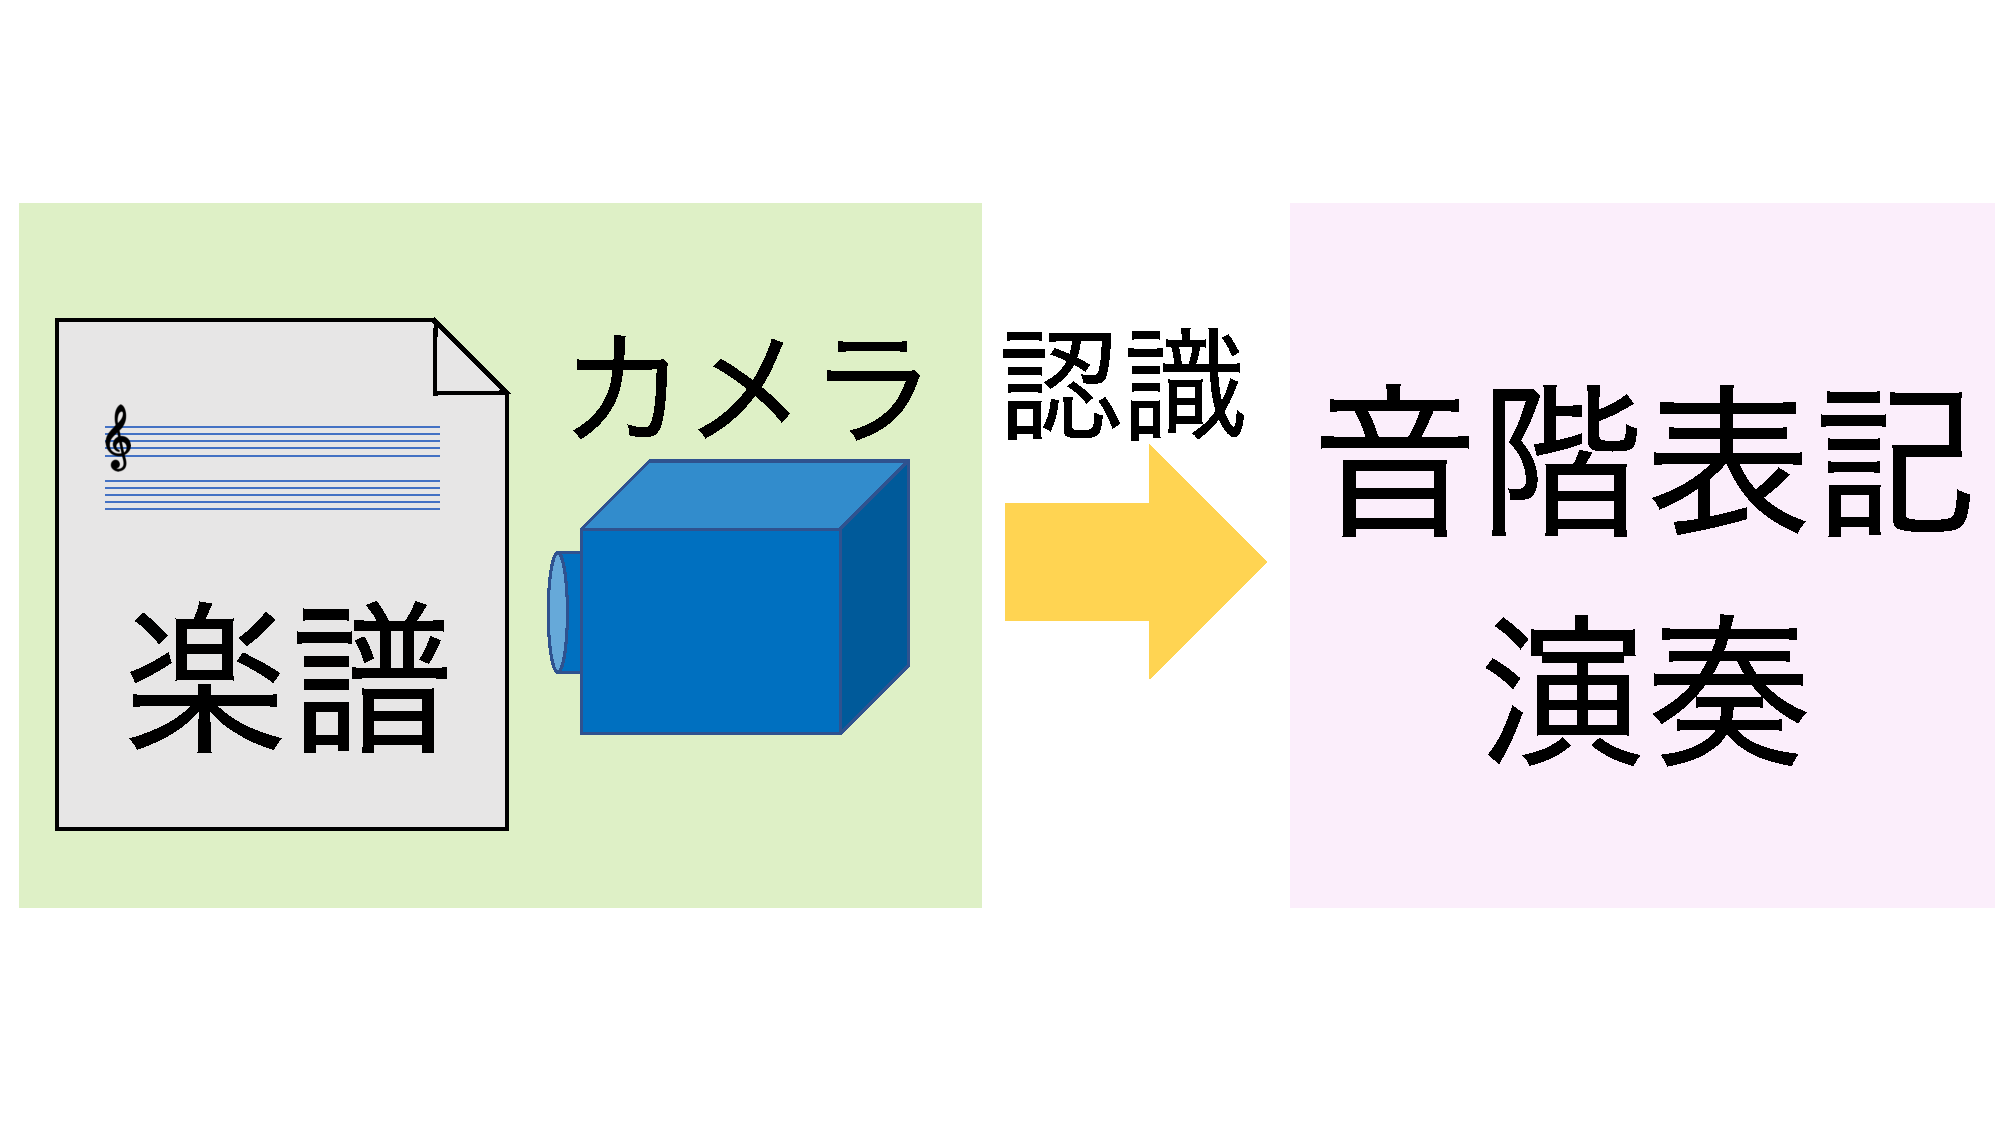
\includegraphics[clip,width=85mm,height=50mm]{image1.pdf}
\end{center}
 \caption{指導者支援システム概要}
 \label{fig:教科書}
\end{figure}

%音情報について
また,現在演奏箇所は赤い線で表記をし,楽譜の上段・下段の差異を視覚化する.
分析した各音符にMIDIで音情報を付与することで視覚だけではなく,聴覚のサポートも行う.システムの画面イメージを図2で示す.

\begin{figure}[h]
\begin{center}
 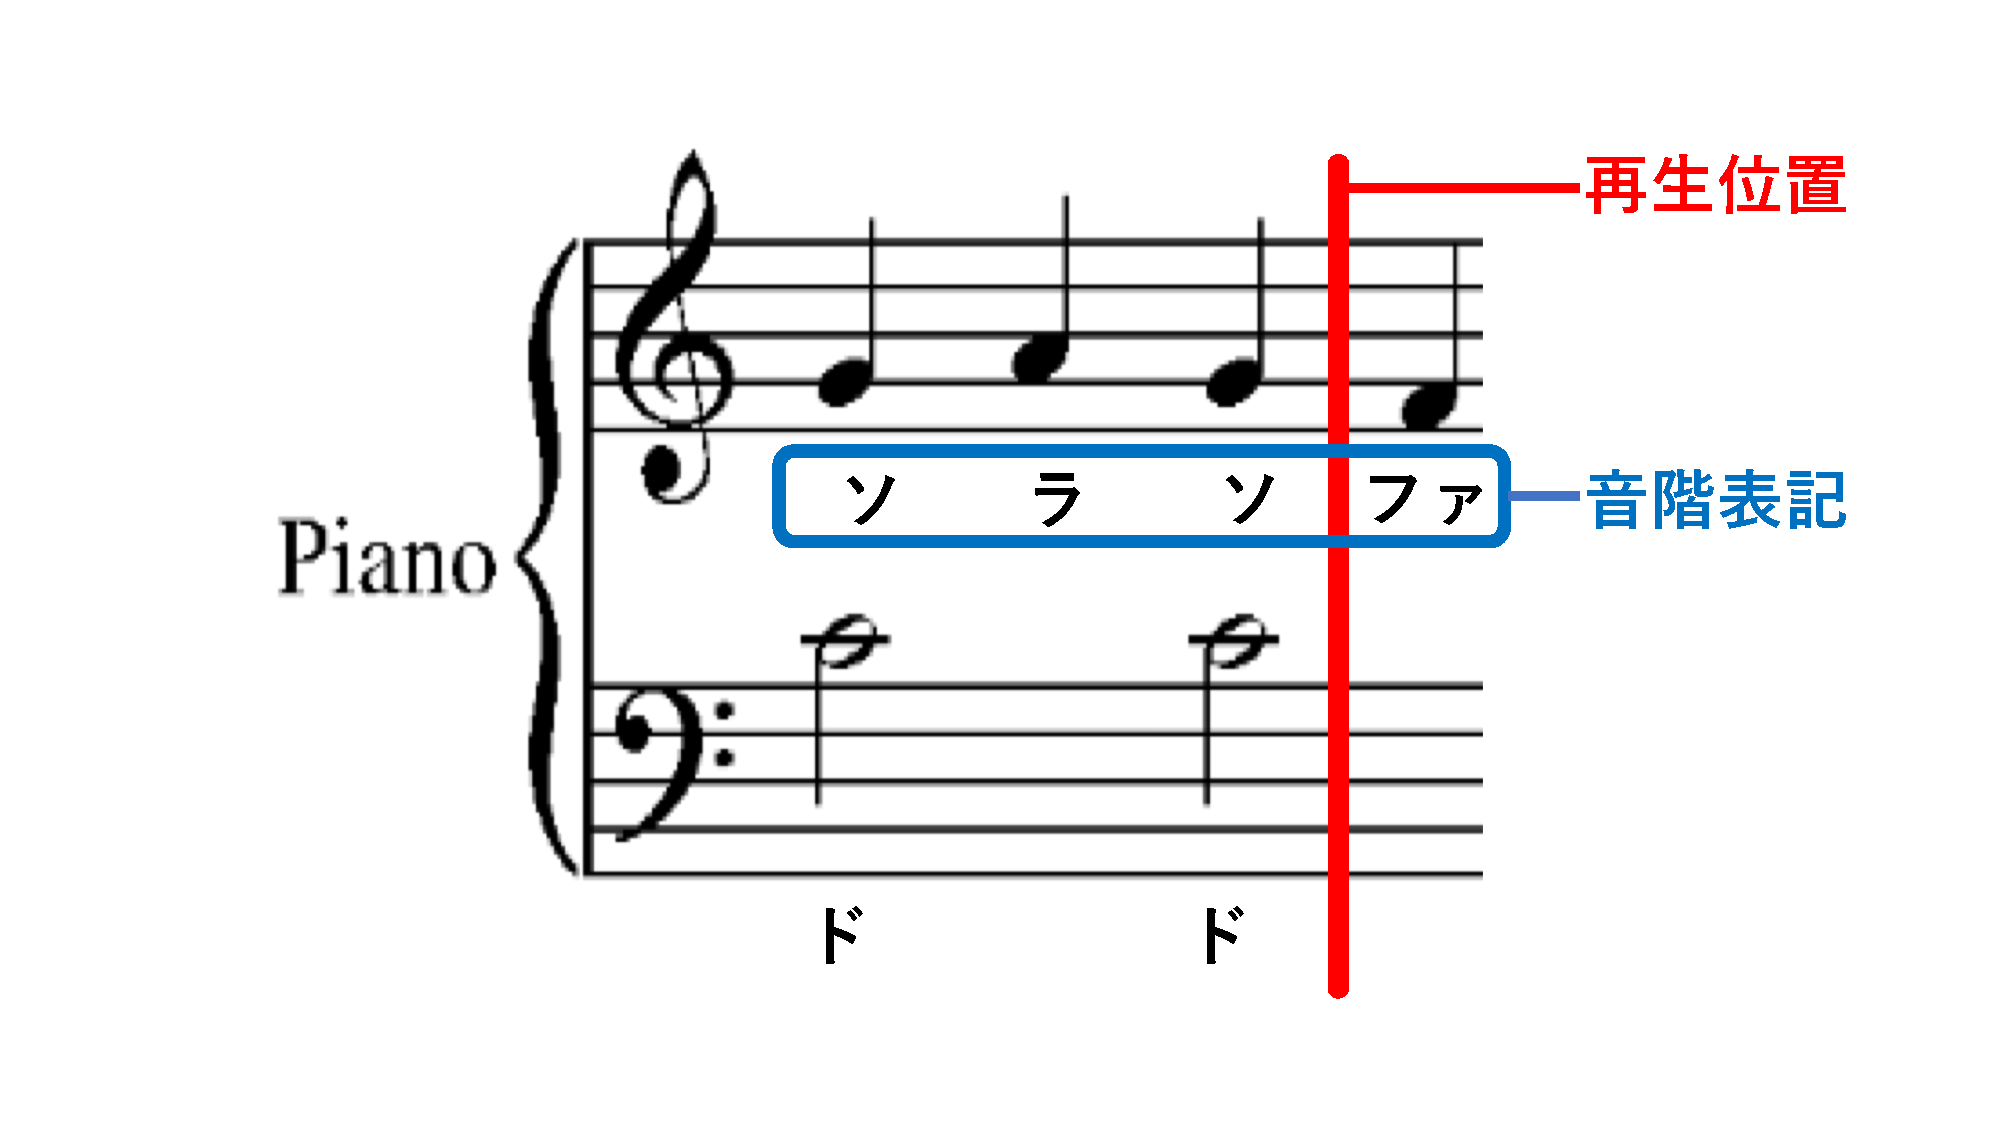
\includegraphics[clip,width=85mm,height=50mm]{image2.pdf}
\end{center}
 \caption{画面イメージ}
 \label{fig:教科書}
\end{figure}

また,楽譜によっては音符に変化記号がついているものがある.変化記号とは,シャープ(♯)やフラット(♭)といった,音を半音単位で高くしたり低くするための記号である.初心者にとって変化記号は見逃してしまうことが多い.そのため,変化記号がついている音階をわかりやすく表記する機能を実装する.

\section{今後の予定}
実際にシステムを制作し,それをピアノ指導者に評価してもらうことで有用性の検証を行う.

\begin{thebibliography}{99}
\bibitem{suda2018} 総務省: ``平成28年社会生活基本調査-生活行動に関する結果-'', \url{http://www.stat.go.jp/data/shakai/2016/pdf/gaiyou.pdf}, (参照 2018-8-23)

\bibitem{suda2018} 政府統計の総合窓口 e-Stat: ``「社会生活基本調査」における「趣味娯楽=楽器演奏」の行動者率(全国集計)'', \url{https://www.e-stat.go.jp/dbview?sid=0003192947}, (参照 2018-8-23)

\end{thebibliography}


\end{document}